\begin{figure}
	\centering
	\begin{subfigure}{0.5\textwidth}
		\centering
		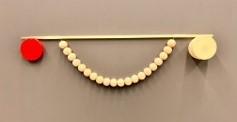
\includegraphics[width=1\textwidth]{papers/kettenlinie/images/kettenlinie_holz.jpg}
		\caption{Kette aus Holz}
		\label{fig:kettenlinie-materialien-holz}
	\end{subfigure}\hfill
	\begin{subfigure}{0.5\textwidth}
		\centering
		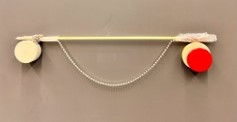
\includegraphics[width=1\textwidth]{papers/kettenlinie/images/kettenlinie_metall.jpg}
		\caption{Kette aus Metall}
		\label{fig:kettenlinie-materialien-metall}
	\end{subfigure}
	\caption{Kettenlinie für Ketten aus verschiedenen Materialien
	\label{fig:kettenlinie-materialien}}
\end{figure}
